\documentclass[a4paper, 12pt]{article}

\usepackage{amsthm, amsfonts,amssymb,epsfig,amsmath,minted,graphicx,hyperref}
\usepackage[margin=0.5in]{geometry}

\setlength\parindent{0pt}

\title{\textbf{CMPE 121 Lab Project} \\ 
    \textbf{Othello (Reversi) for the PSoC-5 Microcontroller}}
\author{Amlesh Sivanantham \\ (asivanan) \\ 1388793}
\date{December 6, 2016}

\begin{document}
	
	\maketitle

	\section{Introduction} 

	The purpose of this lab project was to implement a fully functioning
    game called Othello (Reversi) on the PSoC-5 Microcontroller which built
    on everything we have learned up to this point in the class. The goals at
    the end of the final project were that we would have learned to create
    a functioning hardware and software component. I will go over the whole
    process and go over core functionality of the project in the order that I
    implemented it. However, I will start by explaining the process of
    setting up the hardware first, but it should be noted that each hardware
    component was built only when it came time to implement it in software.
    There are many features that I wanted to implement as well, but do to time
    constraints I was unable to start them. I will ultimately finish
    the features I didn't implement over the winter break. I will go over the
    details of what those features are in the Conclusion section.

    \section{Hardware Design}
 
    There were three components that were required to be connected to the
    microcontroller for this project. They were the RGB LED Matrix, Wifi
    Controller, and the SD Card Reader. As mentioned before, each part was
    only implemented when it came to implement it's respective software
    component. However, It should be noted that first, the breadboard
    was used to prototype the component and test it with the code. Once that
    was verified, it was verified that it was working correctly, the
    components were soldered onto the Perf Board provided to us in the Lab
    Kits. All initial schematics were drawn by hand. 
    \\ \\
    This class was the first time I was introduced to soldering, so I was
    bound to make a mistake. In the process of soldering I made bad
    connections and burnt myself once. This was alright however since I was
    able to verify the my circuit with continuity checks. I had to get a
    replacement SD Card Reader however. In the process of soldering, I
    initially placed the pins the wrong way. Removing the pins was literally
    impossible, but eventually I was able to remove the pins. However there
    was still some leftover solder covering the holes where the pins should
    go. Hence I needed to use the soldering iron and the solder remover to
    remove that remaining solder. Sadly, in the process of removing the
    solder, I managed to burn away the metal plate. Luckily BELS was kind
    enough to allow me to get it replaced for free (it is \$10 normally).
    
    \clearpage
    Seen below are pictures of the schematic and actual perf board after
    soldering was finished.

    \begin{figure}[H]
        \centering
        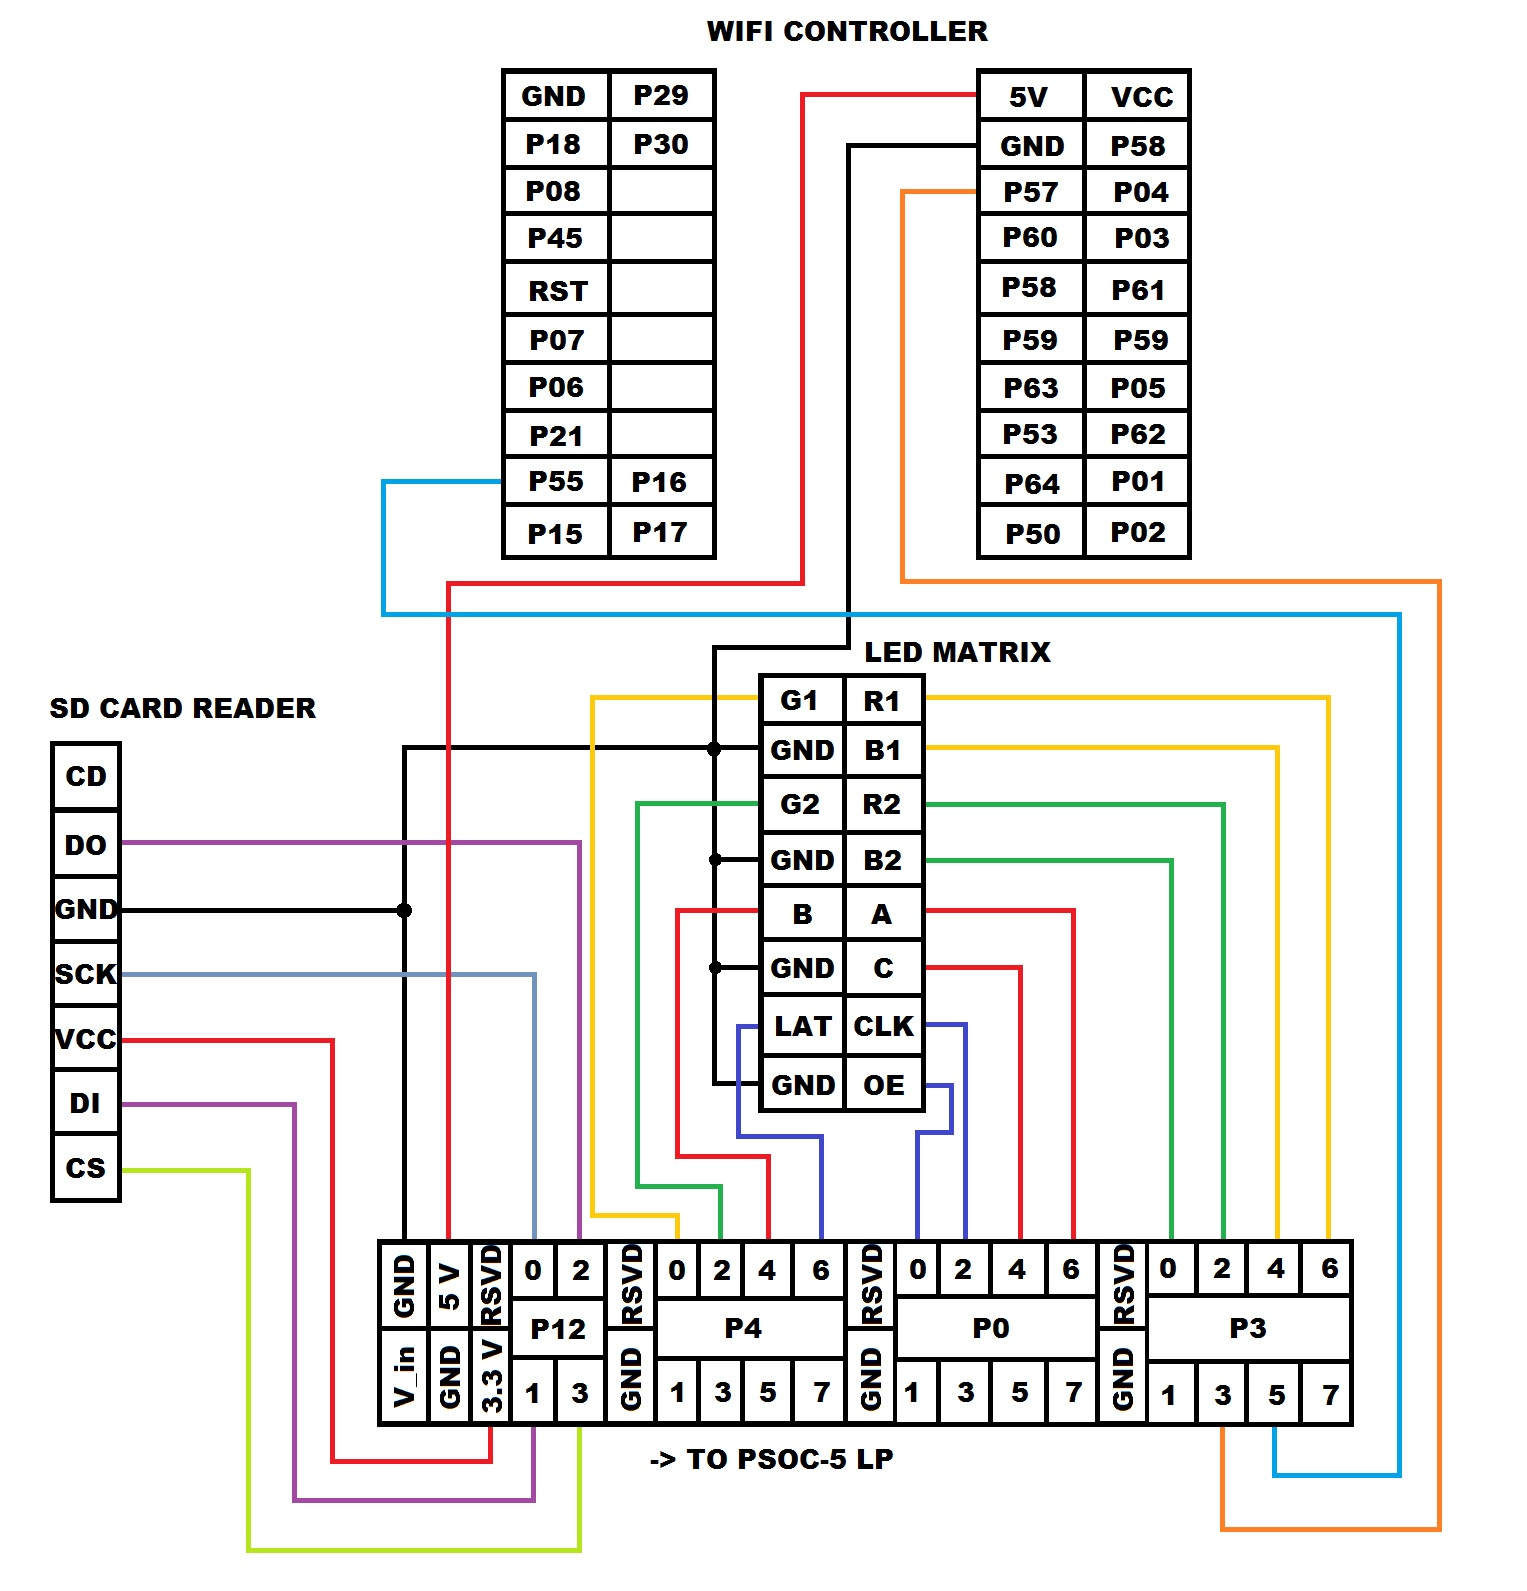
\includegraphics[scale=0.3]{pics/perf}
        \caption{A rough schematic of the connections found on the Perf Board}
        \label{fig:SolderSetup}
    \end{figure}

    \begin{figure}[H]
        \centering
        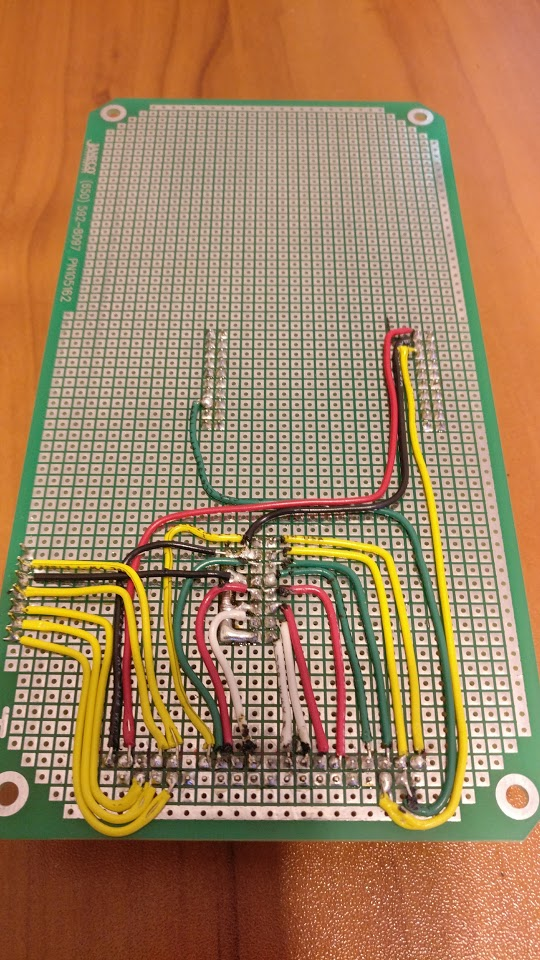
\includegraphics[scale=0.3]{pics/perfBoard}
        \caption{A look at the actual Perf Board}
        \label{fig:PerfSetup}
    \end{figure}

    \section{Software Design}

    \subsection{Workflow and Overview}

    For this lab, I initially made a flowchart of how I wanted to proceed.
    Originally, I made the flowchart on paper, but for the sake of
    convenience, I have made it digital. You can see it below. For each
    section I have made a list of high level goals that I wished to
    implement. Unfortunately, I was not able to get to all of them. 

    \begin{figure}[H]
        \centering
        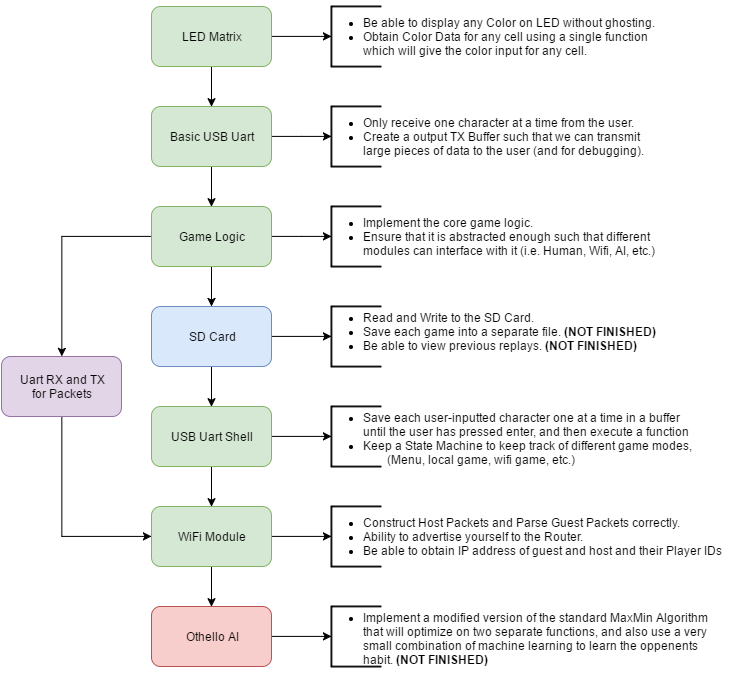
\includegraphics[scale=0.6]{pics/othelloFlow}
        \caption{Overall High Level FlowChart}
        \label{fig:PerfSetup}
    \end{figure}

    Essentially I setup a header file for each module to keep things
    abstracted. In the next few sections I will go over these modules and
    their functionality and constraints, but before we proceed, we will need
    to understand what the file \textit{main.c} does. I wanted my main file
    to be as simple as possible and wanted it behave exactly like the
    picture below.

    \begin{figure}[H]
        \centering
        \includegraphics[scale=0.6]{pics/mainFlow}
        \caption{Structure of Main}
        \label{fig:PerfSetup}
    \end{figure}

    Making my main behave as such allowed me to make things very modular and
    guaranteed a very stable behavior of the program. This also made my
    \textit{main.c} file very small as you can see below.

    \begin{minted}{C}
int main()
{
    
    // Enable Global Interrupts
    CyGlobalIntEnable;
    
    // Start Devices
    LCD_Start();
    
    // Start Init Functions (look at respective header files)
    game_board_reset();
    led_matrix_init();
    usb_uart_init();
    packet_com_init();
    
    // Main Program Loop
    for(;;) {
        
        // Get updates from the Computer Host
        usb_uart_pull();
        
        // Update the current game state
        shell_update();
        
        // Send Feedback to the Computer Host
        usb_uart_push();
    }
    
}
    \end{minted}

    \subsection{LED Matrix (\textit{led\_matrix.h})}

    The LED Matrix is handled very easily. It is triggered via the timer
    interrupt that we say at the top level. It works very much the same way
    that it did in Lab 5, but it gets its color data from a color function
    that has been designed elsewhere. This code is also nearly 100\% modular.
    The only change to port the code elsewhere is to the change the color
    data function. The color data function should take in an input for the
    absolute row and column number and it should figure out what color to
    actually display there. This was done to avoid timing issues. It may be
    a little slower, but it still proved to be a viable method for updating
    the screen while producing no ghosting. The color function will be
    covered in the section pertaining to game logic.

    \subsection{USB Uart (\textit{usb\_uart.h})}

    The primary goals of this module is to get byte data from the user and
    push multiple strings of data back to the user. This is all done with
    four functions and with two buffers. The first buffer is the RX Buffer
    which is defined as \textit{usbDataRX[64]}. The function that we saw
    earlier, \textbf{usb\_uart\_pull()} will update the contents of this
    buffer if possible. It does not append to the end of the buffer, but
    instead it will completely overwrite the RX Buffer. We only wish to
    read in a single user-byte at a time. So we will only look at index zero
    for data. This is done via the function \textbf{usb\_uart\_get()}.
    This is because we are assuming that the USB-COM program on
    the other end is always transmitting bytes the moment a keyboard input is
    pressed (coolterm). Seen below are those very functions.

    \begin{minted}{C}
void usb_uart_pull() {
        
    if(USBUART_GetConfiguration()) {
        
        // If data is ready to be recieved
        if(USBUART_DataIsReady()) {
            
            // get dat data
            usbDataSize = USBUART_GetAll(usbDataRX); 
            
            // if there is anything, set the proper flags
            if(usbDataSize) {                
                newDataRX = 1;
            }
        }
    }
}


// Pull data from the usbData array
//      See if there is new data
//      If there is send it else
//      sends an n

char usb_uart_get() {
    if(newDataRX) {
        newDataRX = 0;
        return usbDataRX[0];
    }
    else
        return 0;
}
    \end{minted}

    While we are processing to the core functionality of the game, we probably
    want to tell the user various information. Thus we will want to create a
    function that will constantly print strings. However, due to the nature of
    the main function, we want to print out after the game update functions
    happen. Thus we will need to create a lot of TX Buffer; in our case, we have
    defined it as \textit{usbDataTX[64][64]}. By creating a function called
    \textbf{usb\_uart\_commit()} which takes in a pointer to a character
    array, we can add data to the TX Buffer. And as seen in the main function,
    we can then use \textbf{usb\_uart\_push()} to push the data that is
    present in the TX Buffers.

\begin{minted}{C}
// Commits data into the TX Buffers
void usb_uart_commit(char* data) {
    int index = 0;
    
    for (index = 0; index < 64; index++) {
        usbDataTX[newDataTX][index] = data[index];
        if(data[index] == '\0')
            break;
    }
    
    if(index) {
        usbDataTXsize[newDataTX] = index;
        if(newDataTX < 64)
            newDataTX++;
    }
}

// Send data from the usbData array
//      See if there is data to
//      transmit. If there is,
//      Send the data back to
//      the host.

void usb_uart_push() {
    uint8 count = 0;
    
    for (count = 0; count < newDataTX; count++) {
        
        while (!USBUART_CDCIsReady()) {}
        USBUART_PutData(usbDataTX[count],usbDataTXsize[count]);
        
        if(usbDataTXsize[count] == 64) {
            while (!USBUART_CDCIsReady()) {}
            USBUART_PutData(NULL, 0u);
        } 
    }
    newDataTX = 0;
}
\end{minted}

    With these functions out of the way, we can proceed to working on other
    parts of the program. The reason why this module was implemented first
    was because in order to test game logic, we will require user input, and
    this module also opens up the ability to error check the code with ease.
    You will notice that in later functions, there be commented out code
    that will be just be a calling \textbf{usb\_uart\_commit()} to print
    data back to the host. If we take a look back at our main function, you
    will notice that we have essentially created the behavior that we
    wanted. 
    \\ \\
    You will also notice the update function in the middle,
    \textbf{shell\_update()}. For the sake of understanding the game logic, let
    us assume that it directly calls the function \textbf{game\_logic\_update()} from the
    file \textit{game\_logic.h}. The shell is essentially a layer above the
    game logic core code. Its purpose is to control modify various
    environment variables and choose different game types. We will look back
    at it in a later section.

    \subsection{Game Logic (\textit{game\_logic.h})}

    There are a lot of subtle things happening in this module with various
    functions, but for the sake of clarity, we will only cover a few
    functions. The first function we will look at is the initialization
    function, \textbf{game\_board\_init()}. It takes an input board size and 
    constructs a game board that matches those specifications. It essentially
    is a reset function that only resets the data pertaining to the game
    board. Here is the code, a lot of the code has been hidden for the sake
    of understanding certain parts.

    \begin{minted}{C}
// Initializes the board to starting position.
void game_board_init(int board_size) {
    
    .......

    // Reset the player start
    player_cur = BLACK_DISC;
    player_cur_pot = POT_BLACK;
    player_cur_pass = FALSE;
    
    player_opp = WHITE_DISC;
    player_opp_pot = POT_WHITE;
    player_opp_pass = FALSE;
    
    ......
    
    // Update the Boundary threshold values
    colBound = (32 - board_type)/2;
    rowBound = (16 - board_type)/2;
    colBound_R = colBound - 8;
    
    int row = 0;
    int col = 0;
    
    // Clear the board
    for (row = 0; row < 16; row++)
        for (col = 0; col < 16; col++)
            game_board[row][col] = 0;
    
    // Setup the initial pieces
    game_board[7][7] = WHITE_DISC;
    game_board[7][8] = BLACK_DISC;
    game_board[8][7] = BLACK_DISC;
    game_board[8][8] = WHITE_DISC;

    .......
}
    \end{minted}

    The variables \textit{player\_cur} and \textit{player\_opp} and its similar
    variables are essentially variables that hold information on the players.
    After each successful move, the two groups of these variables swap contents.
    This is because every function, such as \textbf{place\_piece()} uses only
    the variable \textit{player\_cur} to figure out who the current player is.
    This makes the those functions much simpler to write and easier to understand.
    The swap happens in the function \textbf{game\_logic\_super\_update()}.
    \\ \\
    The game board is setup so that it always appears on the center of the screen.
    This easily done by maintaining a 16 x 16 grid. However, we wish to know
    what the indicies of the row one and column one are. The variables
    \textit{colBound} and \textit{rowBound} essentially will keep the true
    location of row one and column one for a given board size. Because of the
    centering that we are doing, the locations of the starting piece are 
    initialized to the same place regardless of the given board size.
    This setup will allow us to orientate the locations of pieces of a game 
    board of any even size to the LED Matrix. This is done in the function 
    \textbf{get\_board\_data()}. All this functions does is get a value that
    the LED Matrix wants and figures out if that is part of the board or not.
    If it isn't it still may send back color data, but it depends if its a
    border or a end condition. The function also handles displaying the
    cursor and uses the cursor timer from the top level to create the
    blinking effect.
    \\ \\
    There are various other initialization functions for various game modes
    present in this file but we won't look at those. If we take a look at
    the function \textbf{game\_logic\_update()}, we will notice that it takes
    in the user byte command and tries to figure out if it is a meaningful
    input. Essentially it just calls the function to move the cursor, reset
    the board, pass the turn, and place the piece. If a piece was successfully
    placed or the user passed their turn, the global variable \textit{gameChange}
    will be set to true. This will call the function 
    \textbf{game\_logic\_super\_update()} to switch the players as mentioned
    before.
    \\ \\
    There is a sister function to \textbf{game\_logic\_update()} called
    \textbf{game\_logic\_update\_pve()} which does the same thing but with
    the assumption that there is also an online guest. Here is the code below.

    \begin{minted}{C}
void game_logic_update_pve(uint8 command) {
    
    if (local_turn)
        game_logic_update(command);
    
    else{
        
        player_cur_pass = FALSE; 
        
        game_logic_update_only_reset(command);
        
        gameChange = place_piece_nonlocal(rowBound + guest_row(), 
                                          colBound_R + guest_col(), 
                                          guest_pass());
        
        if(gameChange)
            game_logic_super_update();
    }
}
    \end{minted}

    We can see that is uses the variable \textit{local\_turn} to keep track of
    whether it is the guest's turn or the host's turn. If it is the host's
    turn, it will call the actual \textbf{game\_logic\_update()} function.
    If it is the guest's turn, it will try to get their row and col that
    was obtained from the last good packet received by the board. The packet
    data is always begin updated in the background, but its really only updated
    if the game board guarantees that the packet is not invalid in any way.
    This means that the function \textbf{place\_piece\_nonlocal()} will return
    false if it was not able to place a piece successfully and can only do so
    once the guest has sent a valid packet. The details of this will be 
    covered later. If it does place a piece successfully, then it will also
    allow the function \textbf{game\_logic\_super\_update()} to be called
    which will set the turn back to the host.
    \\ \\
    The function \textbf{game\_logic\_super\_update()} also updates the packet
    data and will swap \textit{player\_cur} family of variables with the
    \textit{player\_opp} family of variables. At the end of this function,
    it checks to see if the double pass win condition has occurred so that it
    can trigger the end game. It also calls the function 
    \textbf{board\_pot\_update()} which goes through the current board and
    recursively marks the locations in which are potential locations using the
    \textit{player\_cur\_pot} which holds the color information for the
    potential locations of that player. As mentioned before, the game is a 16
    x 16 grid which contains the state of pieces. It also has the color
    information stored into it. But the more important thing is that each cell
    in the grid has the type \textit{uint16}. The reason for this is so that
    we can store the color information in the lower 8 bits, and some other
    useful information in the upper 8-bits. Particularly, we will store the
    directions of influence for a particular potential location. That means the
    directions for which that piece will flip other pieces is saved into the
    location. This means that when we are placing a piece, we need only check
    to see if that spot is marked and then traverse in only the locations
    specified by the upper 8 bits. The marking of potential locations is also
    used to see if a packet is valid. If the row and column location do not 
    map to a particular potential location, we can assume that the packet
    received is invalid.

    \clearpage
    \subsection{SD Card (\textit{sd\_card.h})}

    The SD Card Reader was very easy to implement. Using the header file that
    we linked, \textit{FS.h}, this gave us the API we needed to communicate to
    the SD Card reader. The was done by adding the \textbf{EmFile\_1} block
    into the top design and connecting the pins to the right locations. The
    actual functions that were made were very simple. One would initialize
    the SD Card if the user turned it on in the shell, and another would
    turn it off if the user toggled if off in the shell.
    \\ \\
    The remaining two functions are the write and append functions. It will
    take a file name and data string as input. They are coded the exact same
    way and with just one simple change in the \textbf{FS\_FOpen()} function.

    \subsection{Othello Shell (\textit{othello\_shell.h})}

    The purpose of the shell is so that the user can construct complex commands
    for the program to interpret. Essentially, the Shell will keep a buffer of
    the user inputted characters and once there 'Enter' key has been seen, it
    will process the command. The Shell is also a state machine. This will tell
    it where it should send the user inputted byte data. We can see this in
    the code of the function \textbf{shell\_update()} below.

    \begin{minted}{C}
// By the will of the global state machine, I command you!!!
void shell_update() {
    uint8 command = usb_uart_get();
    
    switch(board_state) {
            
        case MENU: 
            //game_menu_update_OUTDATED(command);
            command_update(command);
            break;
            
        case MENU_ADVERT:
            advert_stop(command);
            break;
            
        case ADVERT1:
            advert_stop(command);
            break;
            
        case ADVERT2:
            advert_stop(command);
            break;
        
        case PVP:
            game_logic_update(command);            
            break;
        
        case PVE:
            game_logic_update_pve(command);
            break;
        
        case AVP:
            board_state = MENU;
            break;
        
        case AVE:
            board_state = MENU;
            break;
            
        case END:
            if(command == 'R') {
                usb_uart_commit("Game has been reset!\r\r\r");
                game_board_reset();
            }
            break;           
        
        default: 
            break;
    }
    
}
    \end{minted}

    The \textit{MENU} state is simply the main state of the shell. It will not
    play any game and nor will it display anything besides the user inputted
    byte data. The \textit{MENU\_ADVERT} state is when we are still in the shell
    menu, but we want to see who is advertising over WiFi. The details of this
    will be covered in the next section. The other states are the different
    game modes. Notice how every state has a function (except the 
    unimplemented game modes and END) and each function takes in the byte
    data. This essentially allows each state to process the byte data 
    differently depending on which state it is in. If it is in any one of the
    menu or advertise states, then the command is added to the command buffer.
    Otherwise it will used to give input to the current game.
    \\ \\
    Once the user has pressed the 'Enter' key, the string is parsed and if it
    has a valid command, its corresponding value from the enum
    \textit{SHELL\_COMMANDS} will be returned. Here is the code for the parsing
    function and part of the code of the execute function. The string
    \textit{cmd} is the command buffer.

    \begin{minted}{C}
int command_parse() {
    
    // obtain the number of arguments while parsing each individual argument
    arg_count = sscanf(cmd, "%s %s %s %s %s %s", arg[0], arg[1], arg[2], arg[3], arg[4], arg[5]);
    
    if(!strcmp("reset",arg[0]))
        return Reset;
    if(!strcmp("help",arg[0]))
        return Help;
    if(!strcmp("pvp",arg[0]))
        return Pvp;
    if(!strcmp("pve",arg[0]))
        return Pve;
    if(!strcmp("avp",arg[0]))
        return Avp;
    if(!strcmp("ave",arg[0]))
        return Ave;
    if(!strcmp("clear",arg[0]))
        return Clear;
    if(!strcmp("sdcard",arg[0]))
        return SDCard;
    if(!strcmp("advertise",arg[0]))
        return Advertise;
    if(!strcmp("connect",arg[0]))
        return Connect;
    if(!strcmp("disconnet",arg[0]))
        return Disconnect;
    if(!strcmp("hash",arg[0]))
        return Hash;
    if(!strcmp("bsize",arg[0]))
        return Bsize;
    if(!strcmp("A",arg[0]))
        return A;
    if(!strcmp("ip",arg[0]))
        return Ip;
    
    return 0;
}

void command_execute(int command) {
    
    // random temp variable
    int temp = 0;
    
    usb_uart_commit("\r");
    switch(command) {
        
        // Menu control commands
        
        case Reset:
            usb_uart_commit("Game has been reset!\r\r\r");
            if(arg_count > 1) {
                sscanf(arg[1],"%d", &temp);
                change_board_type(temp);
            }   
            game_board_reset();
            board_state = MENU_ADVERT;
            break;

        .........
            
        case Pvp:
            game_menu_pvp_init();
            break;
        
        case Pve:
            game_menu_pve_init();
            break;
    
        ........

        // Network control Options
        
        case Advertise:
            if(arg_count > 0) {
                copy_host_id(arg[1]);
                
                construct_host_advert(cmd);
                board_state = ADVERT1;
            }
            else {
                usb_uart_commit("Command advertise needs an String argument.\r");
            }
            break;

        .........        

        default: 
            board_state = MENU_ADVERT;
            break;
    }

    reset_advert_buffer_count();
    cmd[0] = '\0';
    arg[0][0] = '\0';
    usb_uart_commit("\r");
}
    \end{minted}


    For Example, if the user inputted 'advertise LESH', we can see how the 
    functions would behave. The parse function would store the string 
    'advertise' in \textit{arg[0]} and 'LESH' into \textit{arg[1]}. Since
    'advertise' is a command, it will return a particular value to the execute
    function. This will trigger the \textit{Advertise} case and will then
    call the function \textbf{construct\_host\_advert()} so that it will
    create the string to send to the wifi card for advertising. The other
    commands  work like this as well.

    \subsection{WiFi Module (\textit{packet\_com.h})}

    The goal of this module is to be able to communicate with the WiFi Board.
    This is done with the help of three interrupts. The first interrupt is the
    \textbf{rx\_interrupt}. We have set up the UART so that it interrupts when
    the RX FIFO is not empty. The next interrupt is \textbf{tx\_allow}. Essentially,
    we only wish to transmit our packet to the WiFi board every 500 ms. What this
    ISR does is prevent the actual transmit ISR, called \textbf{tx\_interrupt}
    to trigger unless 500 ms has passed. The \textbf{tx\_interrupt} itself
    however, can only be triggered if the TX FIFO is empty.
    \\ \\
    The \textbf{tx\_interrupt} ISR is very simple and code can be seen below.

    \begin{minted}{C}
CY_ISR(tx_interrupt) {
    for (tempi = 0; tempi < 4; tempi++) {
        if(pkt_host_data[txcount] == '\0') {
            txcount = 0;
            tx_packet_allow_Write(0);
            
            if(board_state == ADVERT1)
                board_state = ADVERT2;
            
            else if(board_state == ADVERT2)
                pkt_host_data[0] = '\0';
            
            break;
        }
        else{
            Packet_Uart_PutChar(pkt_host_data[txcount++]);
        } 
    }
    
}
    \end{minted}

    The purpose of \textit{ADVERT1} and \textit{ADVERT2} is so that when a
    command is sent to the WiFi card, it is sent twice in case a bad one was
    sent. I was having issues where sometimes bad data was sent to the card
    and it would reply with error messages. This was fixed by sending that
    that packet twice.
    \\ \\

    Th



\end{document}
